\chapter{Preference learning에서 memory policy까지}
\label{bg:chapter-rlhf-memory-policy}

Language model post-training에서 RLHF가 널리 알려졌기 때문에 ``sleep training도 RLHF인가''라는
혼동이 생긴다. RLHF는 가능한 training recipe 하나이고, sleep은 언제 어떤 persistent state를
변환할지를 규정하는 lifecycle이다. 이 장은 preference data가 어떻게 loss가 되고, 그 도구를 memory
controller에 어떻게 제한적으로 재사용할 수 있는지 설명한다.

\section{Preference pair와 reward model}

같은 prompt $x$에 대한 두 response $y^+,y^-$ 중 사람이 $y^+$를 선호하면 pairwise data
$(x,y^+,y^-)$가 된다. \concept{reward-model}{보상 모델} $r_\psi(x,y)$는 보통

\begin{equation}
\mathcal{L}_{RM}=-\log\sigma\left(r_\psi(x,y^+)-r_\psi(x,y^-)\right)
\end{equation}

을 줄여 선호 순서를 학습한다. 그 뒤 language-model policy가 reward를 높이도록 갱신된다.
InstructGPT pipeline은 demonstration 기반 supervised fine-tuning, comparison 기반 reward model,
PPO 기반 RL의 단계를 분리했다 \parencite{ouyang2022instructgpt}.

\concept{rlhf}{RLHF}의 핵심 비용은 preference collection만이 아니다. policy rollout, reward inference,
reference policy와의 KL constraint, value estimation, repeated validation이 필요하다. 사용자별 nightly
memory update에 이 전체 pipeline을 복제하면 비용과 instability가 utility를 넘을 수 있다.

\concept{rlaif}{RLAIF}는 AI feedback을 사용해 label throughput을 높인다. Constitutional AI는
principle에 따른 self-critique와 AI preference를 활용한 접근을 제시했다 \parencite{bai2022constitutional}.
그러나 teacher bias가 자동 확장되므로, memory fact의 truth를 teacher preference와 동일시하면 안 된다.
AI는 summary quality나 scope violation을 제안할 수 있지만 primary evidence와 user consent를 대체하지 않는다.

\section{DPO: RL rollout 없이 preference loss를 쓰는 선택지}

\concept{dpo}{DPO}는 preference objective를 policy와 reference policy의 log-probability 차이로 직접
표현해 별도 reward model과 online policy rollout을 생략한다 \parencite{rafailov2023dpo}.

\begin{equation}
\mathcal{L}_{DPO}=-\log\sigma\!\left(\beta\left[
\log\frac{\pi_\theta(y^+|x)}{\pi_{ref}(y^+|x)}-
\log\frac{\pi_\theta(y^-|x)}{\pi_{ref}(y^-|x)}\right]\right).
\end{equation}

이는 training을 단순화하지만 pair가 나타내는 선호의 품질, reference drift, distribution coverage 문제는
남는다. Sleep-time에서 ``이 summary가 저 summary보다 낫다''는 pair에는 잘 맞을 수 있지만, long-term
utility와 capacity effect까지 자동으로 학습되는 것은 아니다.

\section{Memory controller가 고르는 여섯 종류의 행동}

\concept{memory-routing}{기억 라우팅}은 다음 결정을 하나의 policy surface로 본다.

\begin{enumerate}
  \item \textbf{trigger}: 지금 sleep job을 시작할지 기다릴지,
  \item \textbf{admission}: 새 event를 버릴지 어느 tier에 넣을지,
  \item \textbf{representation}: text, vector, graph, adapter 중 무엇으로 바꿀지,
  \item \textbf{replay}: 어떤 old/new example을 어떤 비율로 읽을지,
  \item \textbf{eviction}: 어떤 item/module을 삭제·압축·demote할지,
  \item \textbf{publication}: 후보를 reject, shadow, canary, promote 중 어디로 보낼지.
\end{enumerate}

이 action space는 크고 일부 action은 되돌리기 어렵다. hierarchical controller가 상위에서 budget과
destination을 고르고 하위 rule이 item selection을 수행하면 audit와 안전 제약을 넣기 쉽다.

\begin{figure}[htbp]
  \centering
  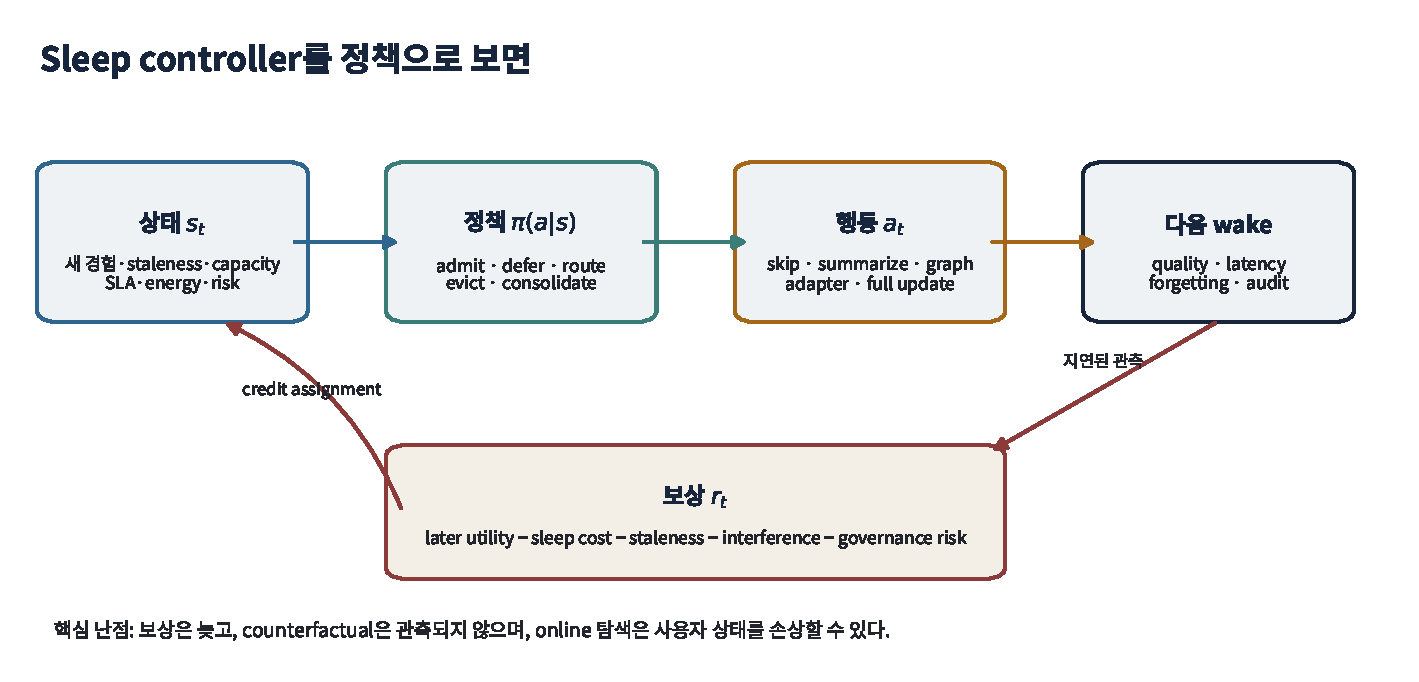
\includegraphics[width=0.94\textwidth]{figures/rl-sleep-policy.pdf}
  \caption{Sleep controller의 강화학습 loop. 실제 보상은 다음 wake period의 utility·forgetting·비용에서
  지연되어 관찰되므로 artifact lineage와 안전한 off-policy evaluation이 필요하다.}
  \figsource{Original synthesis; SRC-STC-0051, SRC-STC-0021}{시스템 상태가 정책으로 들어가고 sleep 행동이 실행된 뒤 다음 wake 결과와 지연 보상이 다시 정책 학습으로 돌아오는 순환도.}
  \label{fig:bg-rl-sleep-policy}
\end{figure}

\section{Offline evaluation이 어려운 이유}

\concept{off-policy-evaluation}{오프폴리시 평가}는 후보 policy를 실제 배포하지 않고 기존 log로
평가한다. 행동 policy $\mu$가 만든 trajectory를 target policy $\pi$에 재가중하는 importance sampling의
기본 형태는

\begin{equation}
\hat V(\pi)=\frac{1}{N}\sum_{i=1}^{N}
\left(\prod_t\frac{\pi(a_t^i|s_t^i)}{\mu(a_t^i|s_t^i)}\right)G_i
\end{equation}

지만 긴 horizon에서는 weight variance가 폭발하고, $\mu(a|s)=0$인 action은 평가할 수 없다. Sleep
action의 downstream utility는 delayed하고 user query가 sparse하므로 model-based simulator와 doubly
robust estimator를 쓰더라도 uncertainty interval을 보고해야 한다.

\begin{table}[htbp]
\centering
\caption{Memory-policy reward를 설계할 때 분리할 signal}
\label{tab:bg-memory-policy-reward}
\small
\begin{tabularx}{\textwidth}{p{0.19\textwidth} X X}
\toprule
Signal & 관측 예 & 잘못 단독 최적화했을 때 \\
\midrule
utility & task success, correction 감소 & benchmark memorization \\
retention & old slice 성능, calibration & 새 변화에 둔감 \\
latency & TTFT/ITL, retrieval hops & 품질이 낮은 aggressive deletion \\
resource & GPU-hour, HBM/SSD bytes, energy & expensive rare capability 제거 \\
governance & scope leak, delete SLA, provenance & 지나친 보수성 또는 미측정 위험 \\
operability & rollback time, version count & 짧은 기간 metric만 선호 \\
\bottomrule
\end{tabularx}
\end{table}

가장 강한 초기 baseline은 learned RL policy가 아니라 explicit rule + constrained optimizer일 수 있다.
RL은 충분한 trajectory coverage와 stable delayed label이 생긴 뒤, trigger와 budget allocation처럼
counterfactual을 시뮬레이션할 수 있는 좁은 action부터 적용한다.
